\chapter{Trash as Medium (Trash in the Art)}

\epigraph{\textit{\quotes{One day, in a rubbish heap, I found an old bicycle seat lying beside a rusted handlebar, and my mind instantly linked them together. I assembled these two objects, which everyone then recognized as a bull’s head. The metamorphosis was accomplished, and I wish another metamorphosis would occur in the reverse sense. If my bull’s head were thrown in a junk heap, perhaps one day some boy would say, \singlequotes{Here’s something that would make a good handlebar for my bicycle!} }}}{\hfill ---Pablo Picasso}

How does trash draw attention of artist(, and also mine)? In this chapter how artist approached to the trash and their techniques are discussed in the context of art. (Historical development, methodologies, tactics, motivations\ldots) Focused on visual (plastic) arts(, because there is also a music genre called as trash music?). How does it turn to medium?

% TODO motivations of artists. their ideas about them, because they also point what is wrong with it? or their perceptions.

%%%
%%%
%%%
\section{Collage, Assemblage and the Found Object}
In this chapter root of using objects in the artworks is examined. Using objects on artworks beyond their intended purpose. Developing artworks not only painting but also using paper and other stuff by pasting them together.

%%
%%
\subsection{Collage}
Collage originates from the French \textit{coller} is an artistic technique of applying manufactured, printed, or “found” materials, such as bits of newspaper, fabric, wallpaper, etc., to a panel or canvas, frequently in combination with painting. In about 1912–13 Pablo Picasso and Georges Braque extended this technique, combining fragments of paper, wood, linoleum, and newspapers with oil paint on canvas to form compositions. Pasting paper is not a new technique but using this it in the art making is a revolutionary movement in the  language of art \cite{waldman1992collage}.

% TODO reading...
\cite{greenberg1984collage}

%%
%%
\subsection{Assemblage}
Assemblage work produced by the incorporation of everyday objects into a composition. It is similar to collage, but main difference is that assemblage is three dimensional rather collage is two-dimensional. Diverse range of things can be used production of work. In 1961, the exhibition "The Art of Assemblage" was featured at the New York Museum of Modern Art. William C Seitz, the curator of the exhibition, described assemblages as being made up of preformed natural or manufactured materials, objects, or fragments not intended as art materials \cite{seitz1961art}.

%%
%%
\subsection{Found Object (Ready-mades)}
Found object originates from the French \textit{objet trouvé}, describing art created from undisguised, but often modified, objects or products that are not normally considered art, often because they already have a non-art function. Pablo Picasso first publicly utilized the idea when he pasted a printed image of chair caning onto his painting titled Still Life with Chair Caning (1912). Marcel Duchamp is thought to have perfected the concept several years later when he made a series of ready-mades, consisting of completely unaltered everyday objects selected by Duchamp and designated as art. The most famous example is Fountain (1917), a standard urinal purchased from a hardware store and displayed on a pedestal, resting on its side.

%%
%%
\subsection{Bricolage}
Something constructed using whatever was available at the time.

Claude Levi-Strauss notes: the bricoleur works not from the principle of making things only if natural resources are available but makes things according to those things at hand, making do with what is available. It is an expression that, like the natural cycles of the Earth, attempts to make something new from something old. \cite{levi1966savage}

% TODO reading...
\cite{strasser1999waste}

%%
%%
\subsection{Folk Art}
In contrast to fine art, folk art is primarily utilitarian(practical and functional, not just for show) and decorative rather than purely aesthetic. The nature of folk art is specific to its particular culture.

Some scholars think that the roots of collage is folk art. (Find resource.) It's methodologies used in this art. The same exist for craft. Some works(for example sculptures from trash) are highly requires craft skills.

%%
%% TODO reading...
\subsection{Art and activism}
Using trash in the art has some critical messages to societies and authorities. Especially in the trash case there is a activist(political) act. 

\subsection{Recycling in the context of Art}
% From Beautiful Trash Art and Transformation BY PAOLA IBARRA, ReVista
Recycling has always been a common practice in the arts at least at a non-material level. From creating a world of words in literature, to rhythm and images in poetry, sampling in hip hop music, representation in the visual arts, or editing the illusory continuity of a film, art implies taking disparate elements (ideas, images, references, objects, etc.) and putting them together to form a new whole. Take and put. De-contextualize and re-contextualize. In that sense, art, as a system, is an act of recycling. 

%%
%%
\subsection{Garbage Art}
"Garbage art (alternatively known as trash art or recycled art) is art created from materials including post-consumer and other waste, collected debris, or objects previously used for other purposes." "Creating art from garbage involves transforming the meaning of objects by placing them in new, aestheticized contexts. This practice is not new; tribal peoples have adapted bits of trash from industrialized societies into their traditional arts since coming into contact with products of the developed world." "Creating art from trash involves “consuming” garbage in the sense that artists appropriate and rearrange the materials in personal ways, transform their meanings, utilize them to their own ends, and represent them in new ways.It involves taking unwanted materials out of their “waste” context and recontextualizing them as “art.”" \cite{tauxe2012encyclopedia}

%%
%% TODO change here
\subsection{History of Consumption and Waste}
"The use of trash as a fine art medium dates back at least to the work of early-20th-century artists such as Fortunato Depero and Kurt Schwitters. Use of found materials, including garbage, has been associated with assemblage art since the 1950s and has been practiced by other well-known artists, including graphic artist Christian Boltanski, sculptor Louise Bourgeois, and photographer Andres Serrano. Art made from garbage has since become much more common in fine arts venues such as museums, galleries, and high-profile installations, including H. A. Schuldt’s famous “Trash People,” which has traveled around the world since 1996." \cite{tauxe2012encyclopedia}

%%%
%%%
%%%
\section{The case of \quotes{The Gleaners and I}}
The Gleaners and I is a 2000 French documentary film by Agnès Varda that features various kinds of gleaning. The Gleaners and I is notable for its fragmented and free-form nature along with it being the first time Varda used digital cameras. This style of film making is often interpreted as a statement that great things like art can still be created through scraps, yet modern economies encourage people to only use the finest product.

It's a self-reflexive film because the director establish a relationship with the practice of gleaners and her film making practice. Some people gleans crops, the others discarded food, the other baby dolls and Agnès Varda gleans images.  

\quotes{Agnès Varda’s film, The Gleaners and I, documents the history and current practice of gleaning in France. Historically, gleaning is the act of collecting leftover crops from farmers’ fields after the harvest. However, in the film Varda expands this definition to include actions that are presently coined \quotes{dumpster diving} where people collect any types of rubbish or unwanted items to reuse them in their own way. Moreover, Varda includes her actions of collecting images with a video camera as gleaning. She is gleaning images. The Gleaners and I far more than document the lives of gleaners. It highlights the degree of global consumerism of the modern world and the ways art can exist within it in relation to gleaning.}

The official subject of this film is gleaning, the act of gathering remnants of crops from a field after the harvest. As Varda demonstrates, people can be discovered throughout the French countryside gleaning everything from potatoes to grapes, apples to oysters, much as they did hundreds of years ago (though no longer in organized groups). More figuratively, there are also urban gleaners who salvage scraps from bins, appliances from the side of the road, or vegetables from stalls after the markets have closed. And then there’s Varda herself, a gleaner of images, driving around France with a digital camera and a tiny crew (at times, she wields a smaller camera herself, permitting an even greater degree of intimacy).

Making use out of something that has been left behind and labeled as obsolete is not unique to farms and crops. There is so much discarded, yet still-viable food in dumpsters that many people live off it entirely. Seeing the value in what someone else has defined as trash is an art in itself.

Once as a common practice of gleaning throughout the years has evolved, but not disappeared. She keeps light to the modern life gleaners that are not visible every time. One of the interesting thing is here Agnès Varda feels that as a aging person will later become discarded person. In other word we can be subject of the refusal. At some point she become the subject of the thing that she track. 

There are many aspects of this documentary film. First draw attention the practice of gleaning. The discarded items that are not fit in the industrial standards because of their shape, color etc. Even if these items are discarded and we are not aware of them, there is also another life for them. Modern life gleaners feed from them. In another words someones trash becomes another trash. There are people live the boundaries of consumption societies. They create their life from the unwanted items. what the society refuses, they find a life or create a life from them. Their lifestyle is also can be seen as alternative to the life on the urban areas with deep relationship with the consumerism. (as also Zizek mentions that love is not idealization. But the industrial processes has some standards and beyond that standards there is not a place for everyone. Life is being lived in the cites is somehow idealized life or tried to be idealized life. beyond the border of the urban there is new life generated. What is not succeed in the cities succeed outside of it.)

She uses unconsciously recorded pieces in the film. \quotes{The last definition of gleaning, gleaning images, ties into what I found both the most amusing and perplexing scene in the film. It is the scene where Varda had forgotten to turn her camera off and accidentally films the ground and her lens cap bouncing along as she walks. She sets this scene to a jazz soundtrack. While watching the scene I was certainly confused. Why is this in here? What does this have to do with gleaning? And certainly why did the scene last so long? But there was also something lovely about it. Maybe it was the music, but for some reasons my senses found it audibly and aesthetically pleasing. I wasn’t able to make much sense out of the meaning behind this scene; I believe Varda referred to it as \quotes{the dance of the lens cap}.  Luckily, Ruth Cruickshank’s article, The Work of Art in the Age of Global Consumption: Agnes Varda’s Les Glaneurs et la glaneuse (The Gleaners and I), addressed this scene and clarified the potential deeper meaning behind it. Cruickshank likened the scene to something that is normally thrown away, or in this case edited out of the film, much like the way trash is thrown away or food is left behind after a harvest. Varda gleans the image of the dancing lens cap, \quotes{Where many documentary makers would leave such accidental footage on the cutting room floor, Varda draws attention to how what would habitually be perceived as waste may be viewed as supplement with its own intrinsic value. Rather than literally treating it like dirt, Varda retains and prompts reassessment of that which is normally left out of shot} \cite{cruickshank2007work}. Things that are often forgotten or discarded can easily be revamped to create something useful to someone. The scene was revamped using music and it became beautiful, much like the gleaners who found fish in the trash cooked it to make it edible, or the artist gleaner who piled discarded baby dolls into totem poles.} 

Refused is not only foods and trash. there are a lot of things that are pushed outside border of the society. She talks and investigates artist that are using discarded items in the artworks. What people not found anything the artist see countless possibilities from them. There is always alternative ways to see something different. Giving life or finding life from discarded life.

The clock found the garbage pile and taken by Agnès Varda. It does not work properly but it has important meaning for her. The time does not go on and it does not remind her that she is aging.

Here another point is that Agnes display images of people picking up things from the ground like their ancestors. Everyone somehow collecting things in their life but particularly she selects these people and their images in action. There should reason for this? For some individuals, gleaning is not a novelty or a clever way to save money, but a necessity of life. They require it to sustain their life. Combine the elements from different peoples that seems totally unrelated gains powerful theme for the documentary. What gleaning means become more open (or powerful). It draws a picture of body combination of different parts (connected, dependent to the each other). The reason of gleaning varies but the fact that gleaning is continues in different forms.

She discusses the importance found in the meaning and purpose of art forms like this: \quotes{Varda seeks to encourage viewers to consider what potential agency is demonstrated in the artfulness and contingency of gleaning by individuals excluded\ldots from the homogenizing systems of global consumption} \cite{cruickshank2007work}. One can find more treasure in trash than many of New York’s finest galleries and art exhibits; they bring a grassroots feel to what has always been seen as a stuffy and prude aspect of society.

The Gleaners And I is not an environmental film. Gleaning, Varda implies, can be understood more broadly as a form of resistance, a way of refusing to be boxed in by conventional expectations; as such, it demands that we re-learn age-old skills as well as supply individual creativity and initiative.

The film tracks a series of gleaners as they hunt for food, knicknacks, thrown away items, and personal connection. Varda travels the French countryside as well as the city to find and film not only field gleaners, but also urban gleaners and those connected to gleaners, including a wealthy restaurant owner whose ancestors were gleaners. The film spends time capturing the many aspects of gleaning and the many people who glean to survive. One such person is the teacher named Alain, an urban gleaner with a master's degree who teaches French to immigrants.

Varda's other subjects include artists who incorporate recycled materials into their work, symbols she discovers during her filming (including a clock without hands and a heart-shaped potato), and the French laws regarding gleaning versus abandoned property. Varda also spends time with Louis Pons, who explains how junk is a "cluster of possibilities." Louis Pons (born 1927) is a French collage artist. He specializes in reliefs and assemblages made entirely from discarded objects and junk. In Agnès Varda's documentary The Gleaners and I, Pons explains his artistic process and understanding of art; what others see as "a cluster of junk," he sees as "a cluster of possibilities;" and that the function of art is to tidy up one's inner and exterior worlds.

%%%
%%%
%%%
\section{Example Artworks}
Artist and artworks related with trash and their analysis. Stages of their works and methods.

% FROM ReVista
Trash is dirty. Trash is smelly. Trash can provide the raw materials for exquisite art---from sculpture to film and beyond.

% FROM Paola Ibarra ReVista
Whether in sculpture, photography or other media, art frequently deals, directly or by allusion, with daily challenges of life in Latin America and elsewhere. Is there a limit to recycling and representation? Or is there a point at which waste cannot become art (or anything else)?

\begin{itemize}
% FROM Maite Zubiaurre, ReVista Garbage
\item Filomena Cruz creates photographic series “Road Kill” painstakingly captures tiny “trash corpses” on the pavement. It is that particular type of trash meet in the public places. trash left behind, trash on the sidewalk, squished, squashed, and weathered. Filomena Cruz sees trash that we don’t want to see. A
piece of chewing gum with an “engraved” leaf; a flattened-out tube; a corroding paper napkin with a still intact heart; or a frog-green Crayola melting in the heat, all speak the language of “worthlessness” suddenly becoming meaningful (and moving).For one thing, trash corpses faithfully record city life. 
  \begin{figure}[ht]
      \centering
      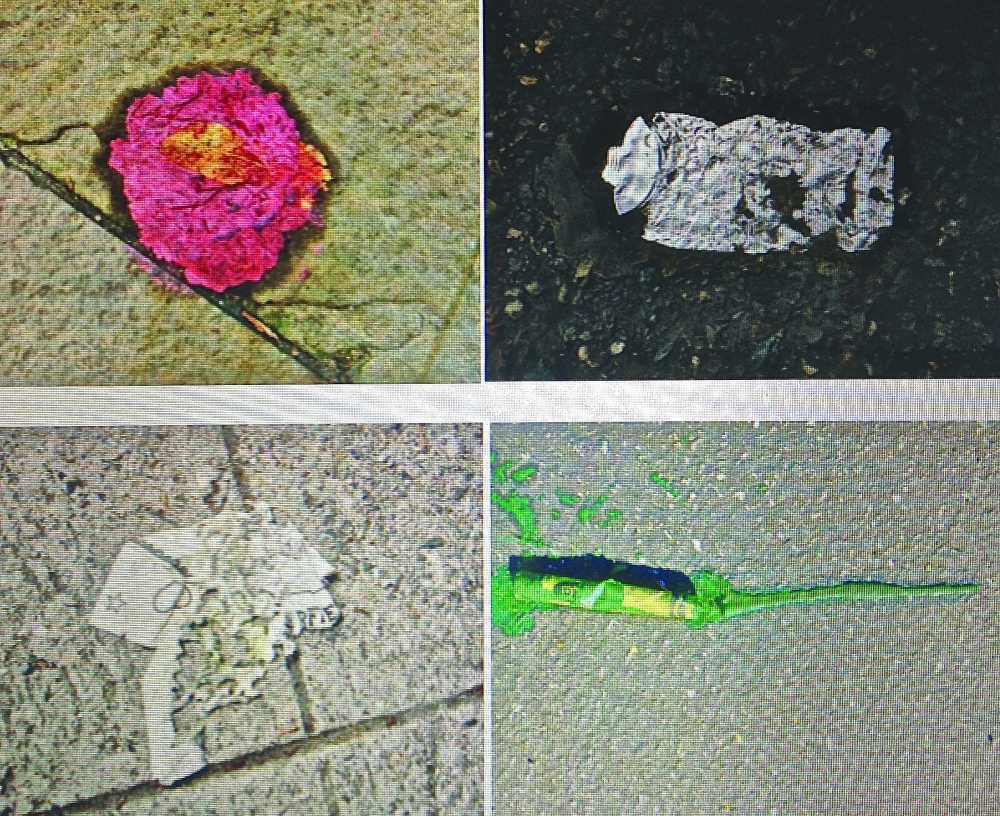
\includegraphics[width=0.8\textwidth]{graphics/FilomenaCruz_RoadKill_ReVista.jpg}
      \caption{Road Kill by Filomena Cruz}
      \label{fig:FilomenaCruz_RoadKill_ReVista}
  \end{figure}

\item Vic Muniz creates monumental trash art in Jardim Gramacho with the help of \textit{catadores} (Waste Land, 2010)

% https://www.youtube.com/watch?v=sJxxdQox7n0
\item Favio Chávez and Nicolás Gómez decide to build musical instruments out of garbage and get 35 children from Cateura, Paraguay’s biggest trash dump, to travel the world with their “Recycled Orchestra,” or “Landfill Harmonic”.

% http://www.eloisacartonera.com.ar/ENGversion.html
\item “Eloísa Cartonera,” a work cooperative in Buenos Aires, proudly produces handmade books with cardboard covers: \quotes{We purchase [\ldots] cardboard from the
urban pickers (\textit{cartoneros}) who pick it from the streets. Our books are on Latin American literature, the most beautiful we had a chance to read in our lives.} \quotes{Some of them are preserved as art books at university libraries, while others circulate as literary pieces expected to disintegrate in time---something anticipated of the material they are made from.} [from PAOLA IBARRA, ReVista]
  \begin{figure}[ht]
      \centering
      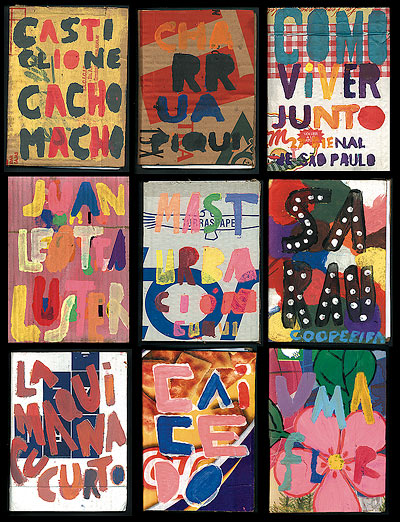
\includegraphics[width=0.8\textwidth]{graphics/EloisaCartonera_Books.jpg}
      \caption{Books covered by Eloisa Cartonera}
      \label{fig:EloisaCartonera_Books}
  \end{figure}

% FROM Paola Ibarra, ReVista
%\item Forever; Blue Yonder by artist Kyle Huffman
%\item Too Too---Much Much by Thomas Hirschhorn
%\item Autoconstrucción by Abraham Cruzvillegas
%\item Pictures of Garbage by Vik Muniz

% FROM Daniel Lind-Ramos BY LOWELL FIET, ReVista
%\item Daniel Lind-Ramos

% FROM A Present from the Sea BY SONIA CABANILLAS, ReVista
% https://www.youtube.com/watch?v=v6IoEF_Tsrw
\item Nick Quijano has some rules to create assemblages. \quotes{There are certain self-imposed rules to this creative process: first, the assemblages or artefactos must all come from material washed ashore on this beach; second, it must be plastic and industrial refuse, result of the processing of fossil fuel; third, it must be polished by a long stay in deep waters, sometimes even encrusted with corals, shells or pebbles, or simply scraped by the ocean floor. As a sign of respect and sacralization, these pieces will be incorporated without any adjustment: no cutting or bending, seen as a mutilation of the object. Its identity cannot be veiled or masked but always must be recognizable amidst the other components; e.g, a comb must remain a comb even as one may see it as a mustache.} The sea returns this refuse; it is not biodegradable.

% FROM Burning Messages BY MICHAEL WELLEN, ReVista
%\item Antonio Berni

% FROM Haiti in the Time of Trash BY LINDA KHACHADURIAN, ReVista
\item Haiti case. When I ask him why he chooses to work in the medium of trash, he replies, \quotes{It gives respect to my city to use the garbage. It shows that everything can be used, and nothing was lost.} (TODO motivation: \quotes{I get more inspiration working with recycled materials because those pieces are unique and can’t be duplicated}) Eugène says that he’s partial to metal, which has become more and more difficult to find because of the clean-up initiative by the city. When I ask him if part of him wishes there were no such effort underway, he answers: \quotes{No. When you have clean streets you have good health, and that is the most important thing.} (This is very strange. It shows that working with trash and being clean healthy is not a contradiction. Both of them exist together.) \quotes{Other people come to Haiti and see junkyards, but we see magical playgrounds,} Jean explains as he watches them.

% FROM Thinking on Film and Trash BY ERNESTO LIVON-GROSMAN, ReVista
% By the 1950s a film like Tire Dié (Fernando Birri, Argentina, 1956) already portrays the collecting, classifying and recycling of trash not only as a source of informal income but as a commercial activity linked to the formal economy. In these films, trash is not the end of a process of consumption but the beginning of a cycle of production. These movies share the idea that trash could be a departure point to think about the modern condition as defined by consumption, class disparities, contamination and urban development. The poet Charles Baudelaire is one of the first to make the connection between the rag picker and the modern city. Walter Benjamin picks it up and from then on the fragmentary condition of trash will remain associated with contemporary art and ultimately with the Modern condition: the industrial refuse could be redeemed by art. It is in this sense that filmmaking becomes allegorical and mimics the process of recycling when it reappropiates archival materials and found footage to create new narratives from scraps, fragments, of films that were not in any way connected to these new narratives.

\item Joseph Cornell

\item \textbf{American Beauty.} The film American Beauty , which features a long, poetic clip of a plastic bag swirling on an eddy of air, snagged five Academy Awards, yet I for one still find it hard to think of plastic bags as things of beauty. 

\item \textbf{Aaron Kramer.} His motto: "Trash is the failure of imagination." \cite{meyer2007turning} In addition to concern for the environment, Kramer was drawn to recycled art because of one simple factor---the price. "Free is certainly great, and that was a driving force for me early on in my career," he said.

\item Nelson’s breakthrough work was The Coral Reef, which he mounted in 2000 at Matt’s Gallery from objects and debris gathered from alleys, trash bins, and car-trunk sales all over London. The title refers to Nelson’s aim of creating an intricate, reeflike network of lives “all existing under one sea, which is capitalism,” he says. (It is very corralate between Ages Varda's work. She shows at the side of human practice, Nelson looks the topic from object side.)

\end{itemize}

Childs can enjoy with trash. I remember from my childhood, we collect crown cap and play with them. Some caps are found less and they worth more. We are looking everywhere for them. To make them flat we put them on the railways. After train passed we get perfect plat cap. At that time it is not trash for us. It has a value and part of our games and enjoy. To have fun a bunch of trash can be enough for us.

In the case of recycling, a dead objects, or an object that reached end of life will begin a new cycle of life. By the artist or other parts are give them a new life. They can reborn as a different things. Do people collect them aware of it? Discarded items unites together with the hands of a artist. 

Trash is global topic men. When you talk about trash, everyone have ideas about it. 

Think a city that has trash monument in the every corner. created from their trash. merged with the city life and gaining unique cityscapes and aesthetics. or think that a museum a trash museum. Exhibits works of art embracing the trash in all aspects. Maybe done by the artist or the visitors from all around world. A place for garbage other than a landfill. Waiting their creator to meet again. What a great idea isn't it? Meeting their creators again. But this time their creator can recognize their trash. They transformed to totally new thing. Reborn. Transformed (Kafka, Gregor Samsa).

%%
%% TODO sample statements here.
\subsection{Artist statements}

\begin{itemize}
\item I am an artist living in New York City, and my experience of daily life here is both the catalyst for and the subject of my art. Working from the local, the personal and the ordinary - the paper take-out coffee cup in the palm of my hand, the view from my studio window in the Garment District, friends and their children, the community garden around the corner from my apartment in Hell's Kitchen - my drawings, paintings and installations are about what happens when the familiar suddenly undergoes a perspective shift and is revealed in all its wonder and infinite possibility. With this shift, mundane things become extraordinary, as nodes of rapidly expanding sets of connections, relationships and new artworks. 

My approach to art-making is both observational and process-oriented. A fascination with cultural, physical and temporal change combined with the possibility of infinite variation unify projects as diverse as drawing and painting on my used coffee cups each day, repeatedly recording the view from my studio in paint and photography over the course of six years, depicting in two and three dimensions the incursion of human activity on the fractal meanders of salt marshes along the New Jersey coast, and painting portraits of alternative families in my New York City neighborhood. (from http://gwynethleech.com/)
\end{itemize}


%%
%%
\subsection{What might be the meaning of using trash as a medium in the artworks? Questioning trash as a medium for artist}
\begin{itemize}
\item Some works try to raise awareness the problems that are the result of trash. (It treats environment and nature.)
\item Some of them reflect people's lifestyle especially throw away culture. As a mirror of current lifestyle.
\item Try to find a new value and meaning from the discarded material that are useless anymore. To explore a new approach, new way. Subvert people's ideas about trash and their attitudes by turning materials to the something meaningful (or valuable). Trash to treasure.
\item Using discarded item to represent other discarded things by the ruling ideology or approach. For example, trash can be used to represent refugees. The things that we are trying to discard does not mean that they have no value, instead it means that we have no ability to reveal its potential. In other words, refugees have potential but we see them as players that will change our current system. Therefore, it can be said that willing to transform trash to treasure is to require change of current lifestyle. Rejecting discarding something especially thing that you get value from it is a process and spread through to the ones life.
\item One way is not to produce trash. (Zero trash philosophy.) The other one is to transform trash into something else.
\item What type of experience is that collecting and working on objects that are generally discarded? Experiencing out of common practice, being open to new explorations.
\item Instead of a world that produce trash, how could it be a world created from trash?
\item Combining industrial goods with objects transformed from trash is another way to find a place to trash in the community. It also signifies that trash still has a good quality to used with new materials. Creating composite products from new and reused items. Using the valuable thing with the invaluable thing. It becomes more valuable or less valuable. Depends on the perception.
\item Aesthetics of trash. Revealing aesthetics value of discarded stuff. (Unique visual value. Trash portraits, sculptures etc.)
\end{itemize}

%%
%%
\subsection{Artistic tactics}

%%%
%%%
%%%
\section{Discussions}
Are artworks made from trash just examples of collage and assemblage or more than from them? What about the experience and interaction with other people? Turning art making process to a life practice (or part of life) can be explained in the context of collage (which is mainly related with how a 2d canvas created). But all of them work in fragments, combine many objects together. 

Garbage is often viewed as a form of society’s excess---as the unwanted things that are thrown out without regard. 

In the world of computer science, the term garbage also refers to situations of loss in which data or objects in memory go unused in computer operations.

(Trash has a history. They have different stories. But same destiny?)

Lets make clear the motto: "trash to treasure". What is treasure here. What does it signify? Treasure---something very valuable. from trash. Then it is trash. Not once it is trash. What type of treasure. Who can get value from it. Who creates this treasure? How does it created? Trash is actually is opposite of treasure and then it is switched. In other words trash become treasure and treasure become trash?

Lets consider the practice of working with trash. Why someone believes that discarded objects of people \ldots Looking things that people are refused. Transforming is the one of the most common practice of whole history of man and nature. This practice is forgotten or it is still alive. Agnes Varda actually shows that it is still exist but in different forms. They use it what ruling lifestyle throw out. They are everywhere actually but you should look them carefully. They live in the borders. But live. Event if they are refused they live. Actually it is hard to say that they want to integrate to the system. They want to change it? 

ability of transform, well actually it is very easy to throw away. hard thing is to keep it. force the material. the dimension of trash.

% FROM drink UP, author: Werthan, Sarah, artist: Leech, Gwyneth. A Year in Cups. http://gwynethleech.com/
% trash and art collided. Paper and art, actually paper already medium of art, but is there anything different here. Itself is a part of a work, not the drawing, or painting.
% Documenting via a blog or a website. (what type of dimension it brings the work? maybe connect them, leave message.)
% Buying a beverage is a daily event for \ldots
% Creating art in public places can demystify the process for passers by, Leech says, making artistic expression more accessible and part of people’s everyday lives.
% “People see that an artist can make work anywhere, and make creative spaces anywhere,” she asserts. 

% Trash is as a material or a subject

\begin{itemize}
\item Where do you think this object came from?
\item Why do you think that someone labeled this object as waste?
\item How can you transform this object to tell the story that you thought of before?
\item What story does it tell you?
\item Does it remind you of an event, a specific time in history or in your life, a place, or a state of mind?
\item How can you bring that story to life? (Taylor, 2006, p. 9).
\end{itemize}

% junkyard art

% TODO PRAP. from rethink, reimagine, reinvent
Recycling art approach to using reclaimed objects in artworks requires rethinking, or examining the affordances of a particular object to explore the possibilities for the object's inclusion in an artwork. Assemblage art involves the creation of new and innovative objects from what were once considered objects of waste; that is. through their use in assemblage pieces, reclaimed objects are endowed with a new. sometimes paradoxical meaning. The transformations of the objects used in assemblage pieces ask viewers to reconsider the notion of "valuable" as they are challenged to look at everyday objects with a new perspective (Taylor, 2006). Viewers confront issues relating to the functionality of objects during modern processes of production, consumption and distribution.

Artifact exploration promotes historical thinking, literacy investigation, and cultural expression (Higgs \& McNeal, 2006; Levstik \& Barton, 2001; Morris, 1998). Meanings are embedded within cultural artifacts and language (Vygotsky, 1978).

%*************************************
% Phrases...
% What specific social issues are you trying to address through Labyrinth?
% In view of the diversity of online crowdsourced art projects, as illustrated by the examples cited so far, it is useful to map out this artistic trend by developing a comprehensive and multidimensional typology of online crowdsourced art. Table 1 organizes this classification according to a set of multiple criteria. (But this one can be used at introduction, but it is too long to fit on introduction. Maybe select works by giving prominence to some of the features. So the approach to the trash is going to be introduced and also it is reveals the what i am doing in this context.) (A Typology of Online Crowdsourced Art. Diye bir örnek var aslında benzer bir şekilde bu trash içinde yapılabilir.) 
\section{Crowdsourcing, Participation}
% TODO needs reference, FROM Crowdsourced Art and Collective Creativity
In the words of Jeff Howe (2006b), the Wired columnist who coined this term in June 2006, \quotes{crowdsourcing represents the act of a company or institution taking a function once performed by employees and outsourcing it to an undefined (and generally large) network of people in the form of an open call}. The vital elements that qualify an outreach strategy as crowdsourcing are, according to Howe, the use of the open call format and the reliance on a large network of potential workers. Although in some cases there is a material reward for the best contributions, the existence of financial incentives is not a required feature in crowdsourcing. Because of the diversity of its applications, crowdsourcing continues to be a disputed term in both the scholarly literature and the popular press; Howe’s original definition is, in this sense, a helpful delineation of its practical sphere.

The value of crowdsourcing lies in the collective intelligence of the contributors. Pierre Levy (1997) describes this concept as “a form of universally distributed intelligence, constantly enhanced, coordinated in real time, and resulting in the effective mobilization of skills” (p. 13). The question of collective intelligence—and its potential efficiency in various practical settings—has received much attention in both academia and journalism. Researchers studying team performance generally agree that, under the right circumstances and with appropriate motivation, large groups of people can work together and harness their collective intelligence to achieve efficient results (Benkler, 2006; Rheingold, 2002; Surowiecki, 2004). Nevertheless, artistic creativity is different from innovation and intelligence, and it requires a unique set of skills and sensibilities as well as a particular type of cultural capital; if we admit that crowds can have collective intelligence, do they also have collective creativity in an artistic sense?

All these pages are rescued and with their [hi]story they are separated from unused new produced blank sheets and notebooks. They are not bought, not gift. They are found. They are accepted. One of the most creative medium is paper and pencil. Chance given to the people through this work.

However, in view of its reliance on the artistic contribution of a large pool of usually anonymous participants, this type of art raises important questions about notions of collective creativity, authorship, collaboration, and the shifting structure of artistic production in the new digital environment. It is well studied area. Pick a method here. Transforming trash with collaboration.

As curator Andrea Grover notes, “having the audience become co-creators is not a new impulse”; the Internet simply offered a new platform to accomplish this goal (Strickland, 2011, para. 5).

Here this question can be raised about why this type collaboration. Another option can be working together with people on a table. Creating things at that time and transforming the objects here. Possibly the connection to the people will more realistic and intense. However same things can be succeed on the internet at some level. 

While crowdsourced art challenges the traditional role of the artist, it simultaneously redefines the conventional function of the public, turning them from passive receivers into engaged producers. (This totally a new area to discuss, I'm going to summarize and introduce concepts and debates. How are they support my work and how they are give way to me?)

% This article therefore aims to fill these critical gaps by analyzing the practice of online crowdsourced art within a framework of collective creativity and participation theories. Principally, my interest is in answering two key questions. What is crowdsourced art and how can it be classified? And how does the structure of the artwork determine the degree or significance of participation?

% discussion is not collaboration, collaboration is used.

% Umberto Eco's Open Work

% SketchBook Project. Inspires me a lot. Lots of works from all over the world. Full of creativity and showcase of richness of people's expressions on the small notebooks. My work can be considered as a sketch book project through trash. Sketches or only creative progress is not the only consideration. You can send your lecture notes. 

% Not all artist transform trash although some deconstruct them. Michael Landy is one of them. 
% Michael Landy's Break Down Inventory is a two week show / display of destruction process of his all possessions on a dissemble line with the help of 10 workers. Firstly they are classified and recorded for three years and the deconstructed in two weeks by separating every element to the smallest part. Reveal all his possessions. and loosing them while you are alive. Turning them to rubbish making them unusable. breaking down the all the meaning. breaking down the connections. 
% Michael Landy's Art Bin uses a art gallery to create his dust bin. Describing the work, simply called Art Bin, as 'about failure', Landy is inviting members of the public to bring their own artistic failures along to the gallery from 29 January, where their worthlessness will be assessed. Damien Hirst, Gillian Wearing, Tracey Emin and Mark Titchner have already contributed, offering sculptures, paintings and prints. "There's no hierarchy once they are in the bin" All of them are accepted as same. Ultimate equality. Tosing them to the dust bin makes them rubbish even if they are combined from failed attempts. Nothing's too good for the art bin. Everything can fit into the art bin. Michael Landy transforms the SLG into Art Bin, a container for the disposal of works of art. As people discard their art works the enormous 600m³ bin becomes, in Michael Landy’s words, “a monument to creative failure”. It is a very big glass bin and isolates people. There is a provocative approach to the art and art objects by saying that "Nothing's too good for the art bin". There is no limitation of throwing away even if art. 

% In this thesis project case the issue is not the nature of art and its methods.

